\documentclass[a4paper,10pt]{article}
\usepackage[utf8]{inputenc}
\usepackage{amsmath, amsthm, amssymb}
\usepackage{color}
\usepackage{systeme}


\usepackage{bbm}
\usepackage{cite}
\usepackage{todonotes}
 \usepackage{empheq}
\usepackage{fixme} 
\usepackage{mathrsfs}

 \usepackage{hyperref}
 \usepackage{subcaption}




\newtheorem{thm}{Theorem}[section]
\newtheorem{cor}[thm]{Corollary}
\newtheorem{lem}[thm]{Lemma}
\newtheorem{rem}[thm]{Remark}
\newtheorem{exa}[thm]{Example}
\newtheorem{defn}[thm]{Definition}
\newtheorem{conj}[thm]{Conjecture}
\newtheorem{prop}[thm]{Proposition}
\theoremstyle{remark}
\newtheorem{comentario}{Remark}


\newcommand{\bm}[1]{\bold{#1}}

%opening
\title{An optimal control problem for a metapopulation SIR model with vaccination}




\author{Gastón Beltritti \\
Dpto. de Matem\'atica,\\ Facultad de Ciencias Exactas, F\'{\i}sico-Qu\'{\i}micas y Naturales\\
Universidad Nacional de R\'{i}o Cuarto\\
(5800) R\'{\i}o Cuarto, C\'ordoba, Argentina,\\
 \\
  Fernando D. Mazzone  \\
Dpto. de Matem\'atica,\\ Facultad de Ciencias Exactas, F\'{\i}sico-Qu\'{\i}micas y Naturales\\
Universidad Nacional de R\'{i}o Cuarto\\
(5800) R\'{\i}o Cuarto, C\'ordoba, Argentina,\\
 \\
}




\begin{document}
\date{}
\maketitle


\begin{abstract}

\end{abstract}


\section{Introduction}
 

The study of epidemic dynamics through mathematical models is an active area of scientific research (see \cite{LindaS.Allen486,FredBrauer478,FredBrauer479,MaiaMartcheva480,FredBrauer482}). The spread of infectious diseases is an extremely complex social and biological process. Numerous factors come into play, including social habits, the level of contact between individuals, public strategies for epidemic mitigation, population structure, information campaigns, demographic changes, and migration. To these must be added factors arising from the interaction between pathogens and the immune system, as well as the evolutionary dynamics of the latter.

It is neither easy nor necessarily useful to construct models that address all of these factors simultaneously. A complex model is more difficult to analyze mathematically, and consequently, it may be challenging to draw clear conclusions from it. Moreover, the practical implementation of mathematical models requires information about the system under study, for example model parameters. These parameters are typically estimated by comparing quantities that can be observed and measured in reality with those that can be computed from the model. This process of fitting the model to empirical data may demand information that is unavailable  in the case of highly complex models.

The objectives of mathematical modeling are also multiple. One critical contribution of this field is providing decision-making criteria, particularly when addressing the allocation of scarce resources. For instance, the development of COVID-19 vaccines occurred concurrently with the 2020–2021 pandemic. During this period, the available stock was inherently limited, forcing health authorities to confront the challenge of optimal distribution across the population



In this article, we investigate the dynamics of epidemics in heterogeneous populations. Heterogeneity means that individuals do not behave in the same way with respect to the progression of the epidemic, and that these differences affect the dynamics of the process. Therefore, assuming homogeneity may lead to inaccurate predictions. A simple example of this situation arises when a disease is transmitted through a network of spatially separated clusters of individuals. It is well known that the transmission of many diseases depends on the level of contact between individuals. In a population structured into clusters, the contact rate of an individual with others in the same cluster is, naturally, expected to differ from that with individuals in other clusters. However, even in populations that are not spatially structured, individuals may play different roles within society, which allows them to be classified into different groups with specific contact rates.

The approach we follow in this article is known in the literature as metapopulation models, or models with patchy environments and movement between patches \cite{FredBrauer482, IstvanZ.Kiss1563, Nowzari2016}.



Vaccines are among the most effective tools for mitigating the incidence of infectious diseases. In some situations, for example during severe outbreaks, the supply of vaccines is limited and decisions must be made regarding their allocation. The objective of this article is to apply the mathematical theory of optimal control to determine the most efficient way to distribute a limited vaccine supply within a metapopulation model. The global vaccination rate is assumed to be a known function of time, and the problem consists of determining how to allocate vaccines so as to minimize a given cost function. In this work, we consider as cost function the total number of infected individuals over the course of the epidemic.

We briefly review some of the literature in which problems similar to those addressed here have been studied.

The so-called complex network epidemiological models \cite{Pastor-Satorras2001,Pastor-Satorras2001b} have received considerable attention. In these models, each individual is represented as a node in a graph. The population is divided into compartments consisting of susceptible individuals, infected individuals, and so on. Moreover, the population is further classified according to the degree (number of neighbors) of the nodes. The resulting model is, in certain respects, equivalent to the one proposed in this article. Structuring the population according to the connectivity of individuals makes it possible to analyze how this connectivity influences the spread of the disease. The analysis of control strategies (quarantine, vaccination, treatment, etc.) on complex networks has been extensively studied in \cite{KANG20173945,Esquivel-Gomez2018,Strona2018,Pastor-Satorras2002,Kalisky2004,Nowzari2016}, among other references.

More specifically, in \cite{Li-2019,rowthorn2009optimal,asano2008optimal,mbah2011resource,Chen-2014,Chen-2014b}, optimal control problems on network metapopulations have been studied. In \cite{rowthorn2009optimal}, an optimal control problem for a metapopulation SIS model with two subpopulations is analyzed. The control strategies considered include treatment and restrictions on inter-population movement, as well as quarantine measures that limit the rate of cross-infection between the two regions. In \cite{asano2008optimal}, a problem similar to the one considered in this article is studied, namely, the optimal distribution of vaccine doses over a network. The objective function in \cite{asano2008optimal} accounts for both the total number of infected individuals and the cost of vaccination. In \cite{Li-2019}, an optimal control problem for a metapopulation SIQS model with quarantine control is studied. In \cite{mbah2011resource}, optimal control is considered for a metapopulation SIR model with treatment and state constraints. In \cite{Chen-2014,Chen-2014b}, optimal control of a metapopulation SIR model with treatment and vaccination is investigated.

One of the main differences between the aforementioned works and the present article is that we do not assume that access to vaccines is limited by their cost; instead, we assume that the vaccine supply itself is limited. More precisely, we assume that the total quantity of vaccines available per unit time for the entire network is given. This leads to what in optimal control theory are known as mixed state-control constraints. In \cite{mbah2011resource,rowthorn2009optimal}, state constraints are introduced in the context of optimal treatment control problems.

We thank S. Aronna for helpful discussions at the X MACI 2025 conference, during which she brought to our attention that the work presented here has significant overlap with \cite{11018532, ARONNA20241198}. In particular, \cite{11018532} considers an optimal control problem concerning the efficient distribution of vaccines in metapopulations under supply constraints. The conclusions obtained in \cite{11018532} are similar to those presented in Section \ref{sec:nece}, namely, that the optimal solution is of bang-bang type. We believe that the present paper complements \cite{11018532}, since our results characterize the nodes where vaccination should be applied in terms of the adjoint variables. Furthermore, we establish several additional mathematical results, including, among others, the existence of endemic equilibria.

 


 


 
\section{The mathematical model}









\subsection{Description and consistency}
By “consistency” we mean that the model admits a unique solution and yields predictions for the variables that are compatible with their biological interpretation.

We consider a population of  $N$ individuals with a common birth and death rate $\mu \geq 0$. We assume that this population is divided into $n$ subpopulations (or nodes) according to a given criterion (geographical location, social activity, number of connections in a complex network, etc). Each subpopulation is further partitioned into susceptible, infected, and recovered individuals, denoted by $S_i$, $I_i$, and $R_i$, respectively. We consider the following network-based SIR epidemic model:

\begin{empheq}[left=\empheqlbrace,]{align}
\label{eq:ModeloSIR1}
    S'_{i}(t)&=\mu N_i-S_{i}(t) \sum\limits_{j=1}^{n} \beta_{i j} I_{j}(t)-  (u_{i}(t) +\mu) S_{i}(t)+\alpha R_i(t) \tag{$P_1$} \\ \label{eq:ModeloSIR2}
    I'_{i}(t)&=S_{i}(t) \sum\limits_{j=1}^{n} \beta_{i j} I_{j}(t)-(\mu+\gamma) I_{i}(t) \tag{$P_2$} \\ \label{eq:ModeloSIR3}
    R'_{i}(t)&=\gamma I_{i}(t)+  u_{i}(t) S_{i}(t)-(\mu+\alpha) R_{i}(t),  \tag{$P_3$}
\end{empheq}
where $i = 1, \ldots, n$ and $N_i = S_i + I_i + R_i$ denotes the total population in node $i$. The parameters in the model have the following meanings: $\beta_{ij} \geq 0$ are the transmission rates from infected individuals in patch $j$ to susceptible individuals in patch $i$; $u_i(t) \geq 0$ (control variable) is the vaccination rate in node $i$ at time $t$; $\gamma^{-1} > 0$ is the average infectious period; and $\alpha^{-1} > 0$ is the average duration of immunity. In Figure \ref{fig:flow_chart}, we present a flow diagram of the model \eqref{eq:ModeloSIR1}--\eqref{eq:ModeloSIR3}.

\begin{figure}[h]
\begin{center}
\def\svgwidth{9cm}
\input{SIR_vacunab.pdf_tex}
\caption{Flow chart of model \eqref{eq:ModeloSIR1}--\eqref{eq:ModeloSIR3}}\label{fig:flow_chart}
\end{center}
\end{figure}

We observe that, by summing equations \eqref{eq:ModeloSIR1}--\eqref{eq:ModeloSIR3} for each $i$, we obtain $N'_i(t)=0$, i.e., $N_i$ is constant in time. Consequently, we can omit equation \eqref{eq:ModeloSIR3} from the system. Therefore, in this article we also consider the following reduced system:

\begin{empheq}[left=\empheqlbrace]{align}
    S'_{i}(t)&=(\mu+\alpha) N_i-S_{i}(t)\left[ \sum\limits_{j=1}^{n} \beta_{i j} I_{j}(t)+ u_{i}(t) +\mu+\alpha\right] -\alpha I_i(t)\tag{$SIR_1$} \label{eq:ModeloSIRb1} \\
    I'_{i}(t)&=S_{i}(t) \sum\limits_{j=1}^{n} \beta_{i j} I_{j}(t)-(\mu+\gamma) I_{i}(t).\tag{$SIR_2$} \label{eq:ModeloSIRb2}
\end{empheq}

In order to address optimal control problems, the control variables $u_i$   are usually assumed to belong to the space $L^{\infty}$, and thus are not necessarily smooth. Hence, it is pertinent to explain in what sense the  functions $S_i$ and $I_i$, $i=1,\ldots,n$ are solutions of \eqref{eq:ModeloSIRb1}-\eqref{eq:ModeloSIRb2}. We must also discuss the conditions under which the initial value problem, associated with the equations \eqref{eq:ModeloSIRb1}-\eqref{eq:ModeloSIRb2}, is well-posed.  

We will adopt the convention of using boldface symbols to denote objects such as vectors and matrices.
Thus, for example, $\bold{\beta}$ denotes matrix $\{\beta_{ij}\}_{i,j=1}^n$, $\bold{S}=(S_1,\ldots,S_n)$ and so on. Given two arrays $\bold{A}$ and $\bold{B}$ we denote by $\bold{A}\times \bold{B}$ the element  wise product of $\bold{A}$ and $\bold{B}$. We write 
\begin{equation}\label{def:x}
\bold{x}=(\bold{S},\bold{I}),\quad \bold{u}=(u_1,\ldots,u_n) 
\end{equation}





\begin{equation}\label{def:func.fS.fY}
    \begin{split}
     \bold{f}_{\bold{S}}&=(\mu+\alpha)\bold{N}-\bold{S}\times (\bold{\beta}\bold{I}+\bold{u})-(\mu+\alpha)\bold{S}-\alpha\bold{I},\\
     \bold{f}_{\bold{I}}&=\bold{S}\times \bold{\beta}\bold{I}-(\mu+\gamma)\bold{I},\\
     \bold{f}&=(\bold{f}_{\bold{S}},\bold{f}_{\bold{I}}),
     \end{split}
\end{equation}
where $\bold{\beta}\bold{I}$ denotes the usual matrix-vector product.

Then the  system  \eqref{eq:ModeloSIRb1}-\eqref{eq:ModeloSIRb2} can be written in compact form $\bold{x}'=\bold{f}(\bold{x},t)$. Given $\bold{x}_0\in\mathbb{R}^{2n}$ we have the corresponding initial value problem

\begin{empheq}[left=\empheqlbrace]{equation}\label{eq:sist_compact}
\begin{split}
 \bold{x}'&=\bold{f}(\bold{x},t).\\
 \bold{x}(0)&=\bold{x}_0
\end{split}\tag{$E$}
\end{empheq}

An aspect that should be noted and that is often neglected in the literature is that the vector field $\bold{f}$ is not continuous. This is because in optimal control problems it is usually assumed that the control functions $u_i$ belong to the space $L^\infty$. Fortunately, we can deal with this type of equation using Carathéodory theory \cite{A.F.Filippov512,EarlA.Coddington236}.
 
Following \cite{A.F.Filippov512} we say that  $\bold{x}$ is a \emph{solution} of \eqref{eq:sist_compact} on an  interval $[0,a)$ if and only if $\bold{x}$ is absolutely continuous on each subinterval $[0,c]\subset [0,a)$, satisfies the initial condition, and $\bold{x}'=\bold{f}(\bold{x},t)$  for almost every $t\in (0,a)$.   Alternatively, this is equivalent to saying that $\bold{x}$ satisfies the integral equation 

\begin{empheq}{equation}\label{eq:eq_integral}
 \bold{x}(t)=\bold{x}_0+\int_0^t\bold{f}(\bold{x},t)dt.
\end{empheq}




We note that if $u_i\in L^1([0,+\infty))$ then $\bold{f}$ is a Carathéodory function in the sense of \cite[p. 3]{A.F.Filippov512} on the domain $\Omega\times[0,+\infty)$, where $\Omega$ is an open and bounded subset of $\mathbb{R}^{2n}$. That means that $\bold{f}(\bold{x},t)$ is continuous in $\bold{x}$ for almost every $t\in[0,+\infty)$,  $\bold{f}(\bold{x},t)$ is measurable in $t$ for each $\bold{x}\in\Omega$ and that there exists a function $m\in L^1([0,+\infty))$ such that $|\bold{f}(\bold{x},t)|\leq m(t)$ for every $(\bold{x},t)\in \Omega\times[0,+\infty)$.   Consequently, we can apply the existence and uniqueness theory for Carathéodory equations \cite[Th. 1, p. 4, Th. 2, p. 5]{A.F.Filippov512}, \cite[Th. 1.1, Ch.2]{EarlA.Coddington236},  and conclude that for any $\bold{x}_0\in \Omega$ there exists a unique local solution of the  initial value problem \eqref{eq:sist_compact}  defined in some interval  $[0,\delta)$, $\delta>0$.




We will use the following well known and elementary formula for the solution of a linear scalar equation of first order $x'(t)+p(t)x(t)=q(t)$:
\begin{equation}\label{eq:1order}
 x(t)=e^{-\int_0^tp(s)ds}\left\{x(0)+\int_0^t e^{\int_0^sp(r)dr}q(s) ds \right\}.
\end{equation}
For $i=1,\ldots,n$ it is convenient to set
\[
 \Theta_i(t):=\sum\limits_{j=1}^{n} \beta_{i j} I_{j},\quad\nu=\mu+\alpha.
\]
Then using formula \eqref{eq:1order} we obtain that equations \eqref{eq:ModeloSIRb1}-\eqref{eq:ModeloSIRb2} and \eqref{eq:ModeloSIR3} are equivalent to the integral equations

\begin{empheq}{multline}\label{eq:eq_integralS}
S_i(t)= \exp\left\{-\nu t- \int_0^t\Theta_i+u_ids\right\}S_i(0)\\
    + 
    \int_0^t \exp\left\{
            \nu (s-t)+\int_t^s\Theta_i+u_idr
            \right\} 
            \left(
                \nu N_i-\alpha I_i
            \right)
            ds 
\end{empheq}

\begin{empheq}{multline}\label{eq:eq_integralI}
I_i(t)= \exp\left(- (\mu+\gamma)t \right)
\left\{  
    I_i(0)+ 
    \int_0^t \exp\left(
            (\mu+\gamma)s\right) 
            \Theta_iS_i
            ds
\right\} 
\end{empheq}


\begin{empheq}{multline}\label{eq:eq_integralR}
R_i(t)= \exp\left(- \nu t \right)
\left\{  
    R_i(0)+ 
    \int_0^t \exp\left(
             \nu s\right) 
            (\gamma I_i +u_iS_i)
            ds
\right\} 
\end{empheq}

 
Equations \eqref{eq:eq_integralS}-\eqref{eq:eq_integralI} have the advantage that they are valid for every $t\geq 0$  while the equations \eqref{eq:ModeloSIRb1}-\eqref{eq:ModeloSIRb2} hold true almost everywhere. 

Although the problem \eqref{eq:sist_compact} makes mathematical sense for any $\bold{x}$ it is only relevant, from an epidemiological point of view, in the closed set
\[
 \Omega_0=\left\{\bold{x}\in\mathbb{R}^{2n}|  0\leq x_i,x_{n+i}\leq N_i, i=1,\ldots,n\right\}.
\]




\subsection{Propagation in the network}

 


In this section, we aim to establish a result concerning the spread of infection in the network.

The following conjecture states that if $\bold{\beta}$ is an irreducible matrix, then the epidemic spreads from any node to the rest with infinite speed. Next, we provide the definition of an irreducible matrix and establish a result that will be useful to prove the conjecture.

\begin{defn}[Reducible and Irreducible matrices]
Let $\bold{\Psi}=\{\psi_{ij}\}_{i,j=1}^n$ be a real matrix. We say that $\bold{\Psi}$ is \textbf{reducible} if there exists a permutation matrix $\bold{P}$ such that $\bold{P}^{T}\bold{\Psi}\bold{P}=\left(\begin{array}{cc}
     \bold{X}  & \bold{Y}\\
     \bold{0} &  \bold{Z}
\end{array}\right)$, where $\bold{X}$ and $\bold{Z}$ are both square matrices. If $\bold{\Psi}$ is not \textbf{reducible} then it is said to be \textbf{irreducible}.
\end{defn}

The following results can be found in \cite{CarlD.Meyer538}.

\begin{lem}\label{lema:Psi.irredusible<-->Grafofuert.conectado}
Let $\bold{\Psi}=\{\psi_{ij}\}_{i,j=1}^n$ be a real matrix. Then, $\bold{\Psi}$ is irreducible if and only if for every pair $(i,j)$, with $1\leq i,j\leq n$ there exists $k_1,k_2,\ldots,k_m\in \{1,2,\ldots,n\}$ such that $\psi_{ik_1}\neq 0$, $\psi_{k_lk_{l+1}}\neq 0$ for $l=1,2,\ldots,m-1$, and $\psi_{k_mj}\neq 0$.
\end{lem}

 

 

\begin{prop}\label{propo:propagacion.en.la.red} Suppose that $\beta$ is an irreducible matrix. If $S_i(0)\geq 0$, $I_i(0)\geq 0$, $R_i(0)\geq 0$ for every $i\in\{1,2,\ldots,n\}$ and there exists $i_0$ such that $I_{i_0}(0)>0$ then for every $i=1,2,\ldots,n$ and $t>0$ we have that $S_i(t)>0$, $I_i(t)>0$ and $R_i(t)>0$; except in the exceptional case where  $\mu=0$, $\alpha=0$ and  there exists $i'$ such that $S_{i'}(0)=I_{i'}(0)=0$, in which case  
$S_{i'}(t)=0$ and $I_{i'}(t)=0$ for all $t\geq 0$.
\end{prop}
 
\begin{proof} 
Let us start with the exceptional case in which $\mu=0$, $\alpha=0$ and there exists $i'$ such that $S_{i'}(0)=I_{i'}(0)=0$. In this case,  the corresponding equations \eqref{eq:ModeloSIRb1} and \eqref{eq:ModeloSIRb2} for $i=i'$ are satisfied by choosing $S_{i'}\equiv 0$ and $I_{i'}\equiv 0$;  thus, in addition, for the other values of $i\neq i'$ we can eliminate the term $\beta_{ii'}I_{i'}(t)$ from the sums in the equations \eqref{eq:ModeloSIRb1} and \eqref{eq:ModeloSIRb2}. That is, we can remove the functions $S_{i'}$ and $I_{i'}$ from the system of equations \eqref{eq:ModeloSIRb1}, \eqref{eq:ModeloSIRb2} and obtain a system equivalent to the original one but with $n-1$ populations. Solving it we obtaining functions $S_{i}$ and $I_i$, for $i\in\{1,2,\ldots,i'-1,i'+1,\ldots n\}$, by adding to these the functions $S_{i'}\equiv 0$ and $I_{i'}\equiv 0$, we obtain a solution of the initial system \eqref{eq:ModeloSIRb1}, \eqref{eq:ModeloSIRb2} with $n$ populations.

Taking into account the previous discussion, we can assume from now on that $\mu>0$, or $\alpha>0$, or for every $i\in\{1,2,\ldots,n\}$ we have that $S_i(0)\neq 0$ or $I_i(0)\neq 0$.

% Before starting to analyze the previous cases note first that if $S_{i}(t)>0$ and $I_i(t)>0$ for every $i\in\{1,2,\ldots,n\}$ and $t\in (0,\delta)$, with $\delta>0$, then $S_i(t)>0$ and $I_i(t)>0$ for all $t\in (0,+\infty)$. In fact, if the last statement were not true taking 

Let us consider the set
$$A:=\{t\in (0,+\infty): S_i(t)\leq 0\ \text{or}\ I_i(t)\leq 0,\ \text{for some}\ i=1,2,\ldots,n\}.$$
It is sufficient to show that $A=\emptyset$. 

Suppose that $A\neq \emptyset$ and define $t_0:=\inf A$.
Note that there exists $j\in \{1,2,\ldots,n\}$ such that $S_j(t_0)=0$ or $I_j(t_0)=0$.  We have two cases. 

\emph{Case $t_0>0.$} 

In this situation we have  $S_i(t)>0$ and $I_i(t)>0$ for all $t\in (0,t_0)$ and every $i=1,2,\ldots,n$. Since $\bold{\beta}$ is an irreducible matrix, we have that for every $i\in\{1,2,\ldots,n\}$ there exists $j_i$ such that $\beta_{i,j_i}>0$. Then $\Theta_i>0$ on $(0,t_0)$, which implies that the integrand in \eqref{eq:eq_integralI} is strictly positive on $(0,t_0)$. In a similar way, we can conclude the same for the integrand in \eqref{eq:eq_integralS}. On the other hand, the term $\nu N_i-\alpha I_i$ is also positive on $(0,t_0)$. Thus $S_j(t_0)>0$ and $I_j(t_0)>0$, which is a contradiction.

\emph{Case $t_0=0.$}

Suppose that $\mu>0$, then $\nu N_i-\alpha I_i(0)>0$ for every $i\in\{1,2,\ldots,n\}$, which implies that $\nu N_i-\alpha I_i(t)>0$ on $(0,\bar{\delta})$ for some $\bar{\delta}>0$. As $S_i(0)\geq 0$ for every $i\in\{1,2,\ldots,n\}$ then, by formula \eqref{eq:eq_integralS}, we have  $S_i(t)>0$ for all $t\in (0,\{\delta\})$ and every $i\in\{1,2,\ldots,n\}$.  

Defining the set $Q_1:=\{i\in\{1,2,\ldots,n\}:\beta_{i i_0}>0\}$, since the matrix  $\{\beta_{ij}\}$ is  irreducible, by Lemma \ref{lema:Psi.irredusible<-->Grafofuert.conectado}, we have that $Q_1\neq \emptyset$. For fixed $i\in Q_1$ we have that $\Theta_i(t)>0$ for all $t\in (0,\delta_i)$ with $\delta_i>0$, and thus $I_i(t)>0$ for all $t\in (0,\delta_i)$.  

For $k\geq 2$, consider the set $$Q_k:=\{i\in \{1,2,\ldots,n\}: i\notin \cup_{j=1}^{k-1}Q_j\ \text{and}\ \exists j_0\in Q_{k-1}\ \ \text{such that}\ \ \beta_{ij_0}>0 \}.$$ Reasoning as before, and by induction, we  see that if  $i\in Q_l$, for some $l$, then $I_i(t)>0$  for all $t\in (0,\delta_l)$ with $\delta_l>0$. 

Since the matrix $\{\beta_{ij}\}$ is irreducible, we have that for every $i\in \{1,2,\ldots,n\}$ there exists $l\in\mathbb{N}$ such that $i\in Q_l$. Thus, we can conclude that $I_i(t)>0$ for all $t\in (0,\tilde{\delta})$, with $\tilde{\delta}>0$, and every $i\in \{1,2,\ldots,n\}$. Therefore, from the previous discussion,   $S_i(t)>0$ and $I_i(t)>0$ for all $t\in (0,\delta)$, for some $\delta>0$, and every $i\in \{1,2,\ldots,n\}$, which is a contradiction with the fact that $0=t_0=\inf A$.

Let us suppose that $\alpha>0$. If $S_i(0)=0$ and $I_i(0)<N_i$ then, by formula \eqref{eq:eq_integralS}, $S_i(t)>0$ for $t\in (0,\delta)$, for some $\delta>0$.  If  $S_{i}(0)=0$ and $I_{i}(0)=N_i$ then, by formula \eqref{eq:eq_integralR},  $R_i(t)>0$ for $t$ close to zero, consequently $\nu N_i-\alpha I_i(t)>0$ near  zero.  Therefore there exists $\delta>0$ such that $S_i(t)>0$ for all $t\in (0,\delta)$ and $i\in\{1,2,\ldots,n\}$. 

Now, reasoning as we did in the previous paragraph, we have that $I_i(t)>0$ for $t$ close to zero and every $i=1,2,\ldots,n$, and we  arrive at a contradiction.  

By last, suppose that for all $i\in\{1,2,\ldots,n\}$,  $S_i(0)\neq 0$ or $I_i(0)\neq 0$. Similarly to the previous argument we can see that $S_i(t)>0$ and $I_i(t)>0$ for $t$ close to zero, and we  obtain a contradiction.
 

\end{proof}


\subsection{Existence of endemic equilibrium}

In this section, we study the existence of equilibria of the model \eqref{eq:ModeloSIR1}-\eqref{eq:ModeloSIR3} when no control strategies are implemented ($\bold{u}\equiv 0$).

Let us first recall the approach to the concept of the \emph{basic reproduction number} by means of the \emph{next generation matrix} (NGM). Following \cite{FredBrauer482}, the next generation matrix for our model is obtained as follows. We write $ \bold{f}_{\bold{I}}=\mathscr{F}-\mathscr{V}$, where $\mathscr{F}=\bold{S}\times \bold{\beta}\bold{I}$ and $\mathscr{V}=(\mu+\gamma)\bold{I}$, and calculate the Jacobian matrices of $\mathscr{F}$ and $\mathscr{V}$ with respect to $\bold{I}$ at the disease-free equilibrium $(\bold{S},\bold{I})=(\bold{N},0)$. We denote by $F$ and $V$ the corresponding matrices. Then the NGM is defined by $K=FV^{-1}$. In the case under study in this section, we have

 \begin{empheq}{equation*}
 K=FV^{-1}=\begin{pmatrix} \frac{N_1\beta_{11}}{\gamma+\mu} & \frac{N_1\beta_{12}}{\gamma+\mu} & \cdots & \frac{N_1\beta_{1n}}{\gamma+\mu} \\
                          \frac{N_2\beta_{21}}{\gamma+\mu} & \frac{N_2\beta_{22}}{\gamma+\mu} & \cdots & \frac{N_2\beta_{2n}}{\gamma+\mu} \\
                          \vdots        & \vdots        &\ddots  & \vdots \\
                          \frac{N_n\beta_{n1}}{\gamma+\mu} & \frac{N_n\beta_{n2}}{\gamma+\mu} & \cdots & \frac{N_n\beta_{nn}}{\gamma+\mu} \\
           \end{pmatrix}.
\end{empheq}
The $(i, j)$ entry of $K$ is the expected number of secondary infections in node $i$ produced by an individual initially in node $j$ (see \cite{FredBrauer482}). The basic reproduction number $\mathscr{R}_0$ is defined as the spectral radius of the matrix $K$, i.e., $\mathscr{R}_0=\rho(K)$, where $\rho(K)$ denotes the maximum absolute value of the eigenvalues of $K$. Observe that if the matrix $\beta$ is irreducible, then the same is true for the matrix $K$; therefore, by the Perron-Frobenius Theorem, we obtain that $\rho(K)$ is itself an eigenvalue. An important fact to remember is that when $\mathscr{R}_0<1$, the disease-free equilibrium is locally asymptotically stable.

In the following theorem, we provide conditions that ensure the existence of an endemic equilibrium, i.e., an equilibrium different from the disease-free equilibrium.

\begin{thm}
 Suppose that there exists $i\in \{1,2,\ldots,n\}$ such that
 \begin{equation}\label{eq:condicion.equilibrio}
A\sum_{j\neq i}K_{ij}N_j<(K_{ii}-1)N_i,
 \end{equation}
 where $A=1+\gamma/(\alpha+\mu)$. Then the system \eqref{eq:ModeloSIR1}-\eqref{eq:ModeloSIR3} has an endemic equilibrium.
\end{thm}
\begin{proof}
 We must find a solution, with $\bold{I}\neq 0$, of
 \begin{empheq}[left=\empheqlbrace,right= \text{, $i=1,2,\ldots,n$}]{align*}
    0&=\mu N_i-S_{i} \sum\limits_{j=1}^{n} \beta_{i j} I_{j}-  \mu S_{i}+\alpha R_i \\
    0&=S_{i} \sum\limits_{j=1}^{n} \beta_{i j} I_{j}-(\mu+\gamma) I_{i} \\
    0&=\gamma I_{i}-(\mu+\alpha) R_{i}
\end{empheq}
Summing the last two equations, we obtain the first one; thus, it is sufficient to solve the second and third equations. If, in the second equation, we replace $S_i$ by $N_i-I_i-R_i$ and $R_i$ by $\frac{\gamma}{\mu+\alpha}I_i$, we get
\begin{equation}\label{eq:F(I)}
\left(1+\frac{\gamma}{\alpha+\mu}\right)\sum_{j=1}^n\beta_{ij}I_jI_i-\sum_{j=1}^n\beta_{ij}I_jN_i+(\gamma+\mu)I_i=0,\ i=1,2,\ldots,n,
\end{equation}
which is a system of $n$ equations with $n$ unknowns (we assume $\bold{N}$ given). We will use the Poincaré-Miranda Theorem, see \cite{PabloAmster218}, Theorem 4.4. We define $F:\mathbb{R}^n\to\mathbb{R}^n$ by means of the expression on the left-hand side of \eqref{eq:F(I)}. We will look for a zero of $F$ in the set $\Omega=[0,N_1]\times \cdots\times [\epsilon,N_i]\times \cdots \times [0,N_n]$ for $\epsilon>0$, which we will specify later. Since $0\notin \Omega$, the zero of $F$ that we will find will be different from the disease-free equilibrium.

For simplicity, we denote by $F_i(I_j=a)$ the result of replacing the $I_j$ component by $a$ in the expression of $F_i$, while the other variables remain arbitrary. In order to verify that the hypotheses of the Poincaré-Miranda Theorem are satisfied, observe that a simple calculation shows that $F_k(I_k=0)\leq 0 \leq F_k(I_k=N_k)$, $k=1,\ldots,n$. This fact is sufficient to apply the above-mentioned theorem, from which a zero of $F$ in $[0,N_1]\times \cdots\times [0,N_n]$ would be obtained. However, this does not exclude the possibility of obtaining the disease-free equilibrium. To overcome this issue, we perform the following calculation
\begin{empheq}{multline*}
 F_i(I_i=\varepsilon)=A\beta_{ii}\varepsilon^2+ \left[A \sum_{j\neq i}^n\beta_{ij}I_j-\beta_{ii}+\gamma+\mu    \right]\varepsilon-\sum_{j\neq i}^n\beta_{ij}I_jN_i\\
 \leq A\beta_{ii}\varepsilon^2+ \left[A \sum_{j\neq i}^n\beta_{ij}N_j-\beta_{ii}N_i+\gamma+\mu    \right]\varepsilon\\
 \leq A\beta_{ii}\varepsilon^2+ (\gamma+\mu)\left[A \sum_{j\neq i}^n K_{ij}\frac{N_j}{N_i}-K_{ii}+1    \right]\varepsilon
 \end{empheq}
Since the term in square brackets is negative, $F_i(I_i=\varepsilon)$ is negative for sufficiently small $\varepsilon$ and for all $I_j$ with $ j \neq i$.
Thus, the hypotheses of the Poincaré-Miranda Theorem are satisfied on $\Omega$, which implies the existence of an endemic equilibrium.

\end{proof}




\subsection{The number of vaccines  for  $t\to +\infty$}
In this section, we assume that the birth rate is equal to zero and the immunity period is infinite, i.e., $\mu=0$ and $\alpha=0$, respectively. The goal is to show that, in some sense, the number of vaccinated individuals at time $t$, $u_i(t)S_i(t)$, approaches zero as $t\to+\infty$ for any $i$, regardless of the vaccination campaign. For example, a very aggressive campaign, so that the vaccination rates $u_i$ are high, will imply that the number of susceptible individuals converges to zero fast enough so that the total number of vaccinated individuals $u_iS_i$ also tends to zero.

What we have actually been able to prove is that certain regularizations of the functions $u_iS_i$ converge to zero at infinity. To state the result that we want to present, let us recall the concept of \emph{regularization} or \emph{approximation of the identity} \cite{EliasM.Stein120}. Let $\varphi$ be an integrable function on $\mathbb{R}$ satisfying $\int_\mathbb{R}\varphi(t)dt=1$. In this article, we only consider functions $\varphi$ such that $\varphi(t)=0$ when $t\leq 0$ and $\varphi$ is decreasing on $[0,+\infty)$. For $\delta>0$, we set $\varphi_\delta(t)=\delta\varphi(\delta t)$ and, for any $f\in L^1(\mathbb{R})$ with $f(t)\equiv 0$ for $t<0$, we write
\[
 f_{\delta}(t)=f\ast \varphi_\delta (t):= \delta\int_{-\infty}^\infty f(t-s)\varphi(\delta s)ds= \delta\int_0^t f(t-s)\varphi(\delta s)ds.
\]

Then it is well known (see \cite{EliasM.Stein120}) that $f_\delta$ is continuous and $f_\delta\to f$ almost everywhere and in the $L^p$-norm with $1\leq p<\infty$.

\begin{comentario}
 Suppose that $f\in L^\infty(\mathbb{R})$ and that there exists $\lim_{t\to\infty}f(t)$. Then, using the Lebesgue dominated convergence theorem, we obtain

 \begin{equation}\label{eq:lim-weak}
 \lim_{t\to\infty}f_\delta(t) =\lim_{t\to\infty}f(t),
\end{equation}
i.e., regularization preserves the limit at infinity.

Nevertheless, the existence of the limit on the left-hand side in equation \eqref{eq:lim-weak} does not guarantee the existence of the limit of $f(t)$ as $t\to\infty$.
\end{comentario}

The following proposition expresses the fact that the epidemic is extinguished as $t\to\infty$ and, in a certain sense, the total quantity of vaccines applied $u_iS_i$ goes to zero as $t\to\infty$.

We recall that $\mu=\alpha=0$ and that the infection period is given by the quantity $\gamma^{-1}$.

\begin{prop} We consider the function $\varphi$ defined by $\varphi(t)=e^{-t}$ when $t>0$ and $\varphi(t)=0$ otherwise. The regularized function $(u_iS_i)_\gamma$ of the total number of vaccines applied at the $i$-th node per unit of time goes to zero as $t\to\infty$. More concretely
\[
 \lim\limits_{t\to\infty}\gamma\int_0^t  u_i(s)S_i(s)
  e^{\gamma (s-t)}ds=I_i(\infty)=0.
\]


\end{prop}

\begin{proof} Adding equations \eqref{eq:ModeloSIRb1} and \eqref{eq:ModeloSIRb2}, we obtain
\[
 (S_i+I_i)'=- u_iS_i-\gamma I_i\leq 0.
\]
Therefore, $S_i+I_i$ is a monotone non-increasing function. Hence, $\lim_{t\to\infty} (S_i+I_i)$ exists. From \eqref{eq:ModeloSIRb1}, the same considerations apply to the function $S_i$. Consequently, there exists $\lim_{t\to\infty} S_i(t)=:S_i(\infty)$. We deduce that there exists $\lim_{t\to\infty} I_i(t)=:I_i(\infty)$. If $I_i(\infty)>0$, we could choose $t_0$ large enough such that $t\geq t_0$ implies $I_i(t)>I_i(\infty)/2=:a>0$. Then $(S_i(t)+I_i(t))'\leq -\gamma I_i(t)\leq -\gamma a$. This inequality implies that $S_i(t) +I_i(t)\to -\infty$ as $t\to\infty$, which is a contradiction. Consequently, $I_i(\infty)=0$.

From \eqref{eq:eq_integralI}, we obtain

\[
\begin{split}
 I_i(t)&=e^{-\gamma t}
 \left\{
    I_i(0)+\int_0^t e^{\gamma s} S_{i}(s) \Theta_i(s)ds
\right\}\\
&= e^{-\gamma t}
 \left\{
    I_i(0)-\int_0^t e^{\gamma s} \left[S'_i(s)+ u_i(s)S_i\right]ds
  \right\}\\
  &= e^{-\gamma t}
 \left\{
    I_i(0)-\int_0^t e^{\gamma s}   u_i(s)S_i(s)ds
    -e^{\gamma t}S_i(t)+S_i(0)+\gamma\int_0^t e^{\gamma s} S_{i}(s) ds
  \right\}\\
   &= e^{-\gamma t}\left(S_i(0)+ I_i(0)  \right)-S_i(t)
   +\gamma \int_0^t e^{\gamma (s-t)}S_{i}(s)ds+\int_0^t e^{\gamma (s-t)}   u_i(s)S_i(s)ds
 \end{split}
\]

The proof is completed by taking the limit as $t\to\infty$ in the previous identities and using \eqref{eq:lim-weak}.
\end{proof}
\section{Optimal control problem}
Before developing the main results of this section, we introduce a more compact notation. The expression $\bold{a}\cdot\bold{b}$ will represent the usual dot product between $n$-dimensional vectors, $\bold{a}$ and $\bold{b}$ , and we will write $\bold{a}>0$ ($\geq$ ) to denote a vector with all positive (non-negative) components.

In this section, we will study the problem of the optimal distribution of vaccines subject to a limited supply of them. By an optimal campaign we mean one that minimizes the total number of infected individuals across all nodes accumulated over a time interval $[0,T]$.  More precisely, given $T>0$, we consider the following Lagrange optimal control problem with mixed inequalities constraints:

\begin{equation}\label{OP:minim}
 \min\limits_{u}\int_0^T\sum_{i=1}^{n} I_{i}(t) d t, \tag{$OP_1$} 
\end{equation}
subjet to:
 


\noindent\textrm{a)} State variable equations

 \begin{align}
    \bold{S}'&=\bold{f}_{\bold{S}}(\bold{S},\bold{I},\bold{u})=\nu\bold{N}-\bold{S}\times (\bold{\beta}\bold{I}+\bold{u})-\nu\bold{S}-\alpha\bold{I},\tag{$OP_2$} \label{eq:OP_2}\\
    \bold{I}'&=\bold{f}_{\bold{I}}(\bold{S},\bold{I},\bold{u})=\bold{S}\times \bold{\beta}\bold{I}-(\mu+\gamma)\bold{I}.\tag{$OP_3$} \label{eq:OP_3}
\end{align}

\noindent\textrm{b)} Initial conditions 

\begin{align}\label{OP:cond.inic}
 \bold{S}(0)=\bold{S}_0>0,\quad \bold{I}(0)=\bold{I}_0,\tag{$OP_4$} 
\end{align}
where $\bold{S}_0$ and $\bold{I}_0$ are known.


\noindent\textrm{c)} Mixed inequalities constraints
\begin{align}
\bold{u}\cdot \bold{S}&\leq M(t)\tag{$OP_{5a}$}\label{res:cant.de.vacunados} \\  
0&\leq \bold{u}.\tag{$OP_{5b}$}\label{res:u>=0}
\end{align}
We denote $\mathcal{U}(t,\bold{S}):=\{\bold{u}:\bold{u}\cdot \bold{S}\leq M(t)\ \text{and} \  0  \leq \bold{u}\}.$





\begin{comentario}
 We emphatize that end point conditions are not given, i.e. $$\bold{S}(T), \bold{I}(T)\ \  \text{free}.$$
\end{comentario}




The objective function in \eqref{OP:minim}
represents $\gamma$ times the total amount of infections in the interval $[0,T]$. Therefore, we are minimizing the latter amount.

The function $M(t)$, which is assumed continuous and greater then zero, has the meaning to being the rate of vaccine supply for the total population at time $t$ per unit of time. Then, the restriction \eqref{res:cant.de.vacunados} means that the total number of vaccines supplied in the network per unit of time does not exceed $M(t)$. 



\section{Existence minimizers}

In this Section, we prove that the problem \eqref{OP:minim}--\eqref{res:u>=0} satisfies the hypothesis of the \emph{Filippov-Cesari Theorem} (see \cite[Th. 9.3.i]{L.Cesari368}), and consequently  it has a solution. 

In what follows, we will use the notation introduced in \eqref{def:x} and  \eqref{def:func.fS.fY}. Additionally we consider the Lagrangian function 

$$
f_{0}\left(\bold{x}, \bold{u}, t\right)=\sum_{i=1}^{n} I_{i}(t).
$$

\begin{thm}
The optimal control problem \eqref{OP:minim}--\eqref{res:u>=0} has a solution $(\bold{x^*},\bold{u}^{*})$.
\end{thm}

\begin{proof}
First we observe that, since $0\leq S_i\leq N_i$, $0\leq I_i\leq N_i$ and $t\in [0,T]$ the domain of the time-state variables can be chosen as a compact set, which we denote by $A$. This fact verifies one of the hypotheses of the Theorem 9.3.i in \cite{L.Cesari368}. 
Additionally,  we need to prove that the set $$ \mathcal{M}:=\left\{(t,\bold{x},\bold{u}): (t,\bold{x})\in A\ \text{and}\ \bold{u}\in \mathcal{U}(t,S)  \right\}  $$ is a compact set in the time-state-control variables space. This fact is true since, from \eqref{OP:cond.inic} and \eqref{eq:eq_integralS} we have that $S_i(t)\geq \delta>0$ for every $t\in [0,T]$, therefore $\mathcal{M}$ is a closed and bounded set, and hence a compact set. Finally, we need to establish that the set $$ \mathcal{Q}(t,\bold{x}):=\left\{(z_0,\bold{z})\in \mathbb{R}^{1+2n}:z_0\geq f_0(t,\bold{x},\bold{u}), \bold{z}=f(t,\bold{x},\bold{u}),\ \text{and}\ \bold{u}\in \mathcal{U}(t,S) \right\} $$
is a convex set, and this is an immediate consequense of the fact that $f$ is a lineal function with respect to the control variable $\bold{u}$.
\end{proof}

\section{Necessary conditions}\label{sec:nece}

In this Section, we apply the Pontryagin Maximum Principle \cite[Th. 4.1]{A.Seierstad499}, \cite{hartl1995survey} for to  obtain necessary conditions  in order to $(\bold{x}^*,\bold{u}^*)=(\bold{S}^*,\bold{I}^*,\bold{u}^*)$ be a solution of the optimal problem  \eqref{OP:minim}--\eqref{res:u>=0}.  

As is well known the maximun principle involves the Hamiltonian formulation of the optimal problem. We consider \emph{adjoint variables},

$$\bold{p}_S(t)=(p_{S1}(t),\ldots,p_{Sn}(t)) \ \text{and}\ \bold{p}_I(t)=(p_{I1}(t),\ldots,p_{In}(t))$$
and the Hamiltonian function defined by
\begin{empheq}{multline}\label{eq:hamiltoniano}
\mathscr{H}(\bold{S},\bold{I},\bold{u},\bold{p}_S,\bold{p}_I)=
-p_0 \sum_{i=1}^{n} I_{i}  
 +\bold{p}_{S}\cdot \bold{f}_{\bold{S}}(\bold{S},\bold{I},\bold{u})+ \bold{p}_I\cdot \bold{f}_{\bold{I}}(\bold{S},\bold{I},\bold{u}),
\end{empheq} 
where $p_0\in\mathbb{R}$ is independent of $t$. It is necessary to introduce  new multipliers  $\bold{q}(t)=(q_0(t),q_1(t),\ldots,q_n(t))$ associated with \eqref{res:cant.de.vacunados}  and \eqref{res:u>=0} respectively and the  \emph{Lagrangian} or \emph{generalized Hamiltonian} $\mathscr{L}$ defined by
\begin{empheq}{equation}\label{eq:lagrangiano_generalizado}
\mathscr{L}(\bold{S},\bold{I},\bold{u},\bold{p}_S,\bold{p}_I,\bold{q})=\mathscr{H}(\bold{S},\bold{I},\bold{u},\bold{p}_S,\bold{p}_I)+(q_1(t),\ldots,q_n(t))\cdot \bold{u}-q_0 \bold{u}\cdot \bold{S}.
\end{empheq} 

We suppose that $(\bold{S}^*,\bold{I}^{*},  \bold{u}^{*})$ is a  solution of \eqref{eq:optimal_model}. From now on any function evaluated at  $(\bold{S}^*,\bold{I}^{*},  \bold{u}^{*})$  will be indicated with a $\ast$ as superscript.

We combine the restrictions in a vector valued function 
$$\bold{h}(\bold{S},\bold{u},t)=(-\bold{u}\cdot \bold{S}+M(t),\bold{u}_1,\ldots, \bold{u}_n).$$
Then, the constraints are expressed synthetically $\bold{h}\geq \bold{0}$, where order relations between vectors mean that these relations are given component by component. Following  to be able to apply the Maximum Principle  it is necessary that they satisfy the  
According to \cite[Th. 4.1]{A.Seierstad499}, see also \cite{hartl1995survey}, in order to apply the maximum principle, the  constraint
qualification condition must be satisfied. This condition  means that the gradients of the active constraints ( this is $ \{i :h_i=0\}$) are linearly. In our case, the following condition must be satisfied

\begin{equation}\label{eq:cons_qua}
n+1=
 \operatorname{rank}
                    \left[
                    \begin{array}{c c c|c c c c }
                      1      & \cdots & 0      & u_1    & \cdots& 0 &  0       \\
                      \vdots & \ddots & \vdots & \vdots & \ddots&\vdots & \vdots   \\
                      0      & \cdots & 1      & 0 &\cdots &  u_n   &   0      \\                                  
                      -S_1   &\cdots  & -S_n      & 0      &\cdots &0 & -\bold{u}\cdot \bold{S}+M(t)\\
                     \end{array}
                    \right]
\end{equation}
We note that if $-\bold{u}\cdot \bold{S}+M(t)\neq 0$ then then qualification condition follows inmediately. In the case that   $-\bold{u}\cdot \bold{S}+M(t)= 0$ (last constraint active) we can  prove  that  the matrix en the rhs of  \eqref{eq:cons_qua} can be row reduced to
\begin{equation*}\label{eq:cons_qua}
                    \left[
                    \begin{array}{c c c|c c c c }
                      1      & \cdots & 0      & u_1    & \cdots& 0 &  0       \\
                      \vdots & \ddots & \vdots & \vdots & \ddots&\vdots & \vdots   \\
                      0      & \cdots & 1      & 0 &\cdots &  u_n   &   0      \\                                  
                      0   &\cdots  & 0      & u_1S_1      &\cdots & u_nS_n & 0\\
                     \end{array}
                    \right].
\end{equation*}
Since $-\bold{u}\cdot \bold{S}+M(t)= 0$, there is some $i$ with $u_iS_i\neq 0$. This implies that matrix has completed rank. 

We are in a position to apply the maximum principle. First we observe 
that in virtue of  equations (29), 
(34) and (35c) in \cite[Th. 4.1]{A.Seierstad499} we can assume  that 
$p_0=1$ in \eqref{eq:hamiltoniano}. On the other hand, we infer that 
there exist
functions $ \bold{p}^\ast_S,\bold{p}^\ast_I:[0,T]\to\mathbb{R}^n$
 and 
\emph{multipliers} $\bold{q}:=(q_0(t),\bar{\bold{q}}(t)):=(q_0(t),\ldots,q_n(t))\in\mathbb{R}^{n+1}$ 
such that  the following 
conditions are satisfied

\noindent 1.\emph{ Adjoint equations}
 
 \begin{subequations}
\makeatletter
\def\@currentlabel{ADJ}
\makeatother
\label{eq:estado_adj}
\renewcommand{\theequation}{ADJ${}_\arabic{equation}$}
\begin{empheq}[left=\empheqlbrace]{alignat=3}
\dot{\bold{p}}_{\bold{S}} 
    &=-\frac{\partial \mathscr{L}^\ast}{\partial \bold{S}}
        &={\bold{p}}_{\bold{S}} \times \left(\bold{\beta} \bold{I}^\ast +\bold{u}^\ast+\nu\right) 
            -{\bold{p}}_{\bold{I}}\times  \bold{\beta} \bold{I}^\ast +q_0\bold{u}^\ast,\label{eq:cons_adjS}\\
\dot{\bold{p}}_{\bold{I}} 
    &=-\frac{\partial \mathscr{L}^\ast}{\partial \bold{I}}
        &= p_0\bold{1}+ \bold{\beta}^t\left( \bold{S}^\ast\times \left( {\bold{p}}_{\bold{S}}-  
            {\bold{p}}_{\bold{I}} \right)\right)
                +\alpha {\bold{p}}_{\bold{S}}+(\mu+\gamma) {\bold{p}}_{\bold{I}},\label{eq:cons_adjI}
\end{empheq}
\end{subequations}
where $\bold{1}=(1,\ldots,1)\in\mathbb{R}^n$.
 

\noindent 2.\emph{ }
 \begin{empheq}{equation}\label{eq:L_critico}
  0=\frac{\partial \mathscr{L}^\ast}{\partial \bold{u}}=
  -{\bold{p}}_{\bold{S}}\times \bold{S}^\ast +\bold{q}-q_0\bold{S}^\ast
 \end{empheq}

\noindent 3.\emph{ Positivity and complementary slackness conditions } 
 \begin{empheq}{equation}\label{eq:rest-act}
  \bold{q}(t)\geq 0 \quad \text{ and }\quad  \bold{q}(t)\cdot 
  \bold{h}(\bold{S}^\ast,\bold{u}^\ast, t)=0
 \end{empheq}

\noindent 4.\emph{ Terminal condition }  

 \begin{empheq}{equation}\label{eq:p-values}
  p_0=1 \quad \text{ and }\quad  \bold{p}_{\bold{S}}(T)= \bold{p}_{\bold{I}}(T)=0.
 \end{empheq}


\noindent 5.\emph{ Maximality. } For fix $t\in[0,T]$ and for 
every $\bold{u}$ with  $\bold{h}(\bold{S}^\ast,\bold{u},t)\geq \bold{0}$\todo{Revisar por que en  \cite[Th. 1, p. 276]{A.Seierstad499} dice  $\bold{h}(\bold{S}^\ast,\bold{u},t)> \bold{0}$} we have
\begin{empheq}{align}\label{eq:maximalidad}
\mathscr{H}(\bold{S}^\ast,\bold{I}^\ast,\bold{u}^\ast,\bold{p}_S^\ast,\bold{p}_I^\ast)\geq 
\mathscr{H}(\bold{S}^\ast,\bold{I}^\ast,\bold{u},\bold{p}_S^\ast,\bold{p}_I^\ast)
\end{empheq}

From the fact that $\boldmath{h}(\boldmath{S},\boldmath{u},t)\geq 0$ and from \eqref{eq:rest-act} we have that if $u_j^\ast(t)\neq 0$ then $q_j(t)=0$. Thus, from \eqref{eq:L_critico}, $q_0S_j^*=-p_{Sj}S_j^*$ when $u_j\neq 0$. Therefore, since $S_j^*\neq  0$ (see Proposition \ref{propo:propagacion.en.la.red}), we can replace equation \eqref{eq:cons_adjS} by 
\begin{empheq}{equation}\label{eq:cons_adjS.prima}
 \dot{\bold{p}}_{\bold{S}} 
    ={\bold{p}}_{\bold{S}} \times \left(\bold{\beta} \bold{I}^\ast +\nu\right) 
            -{\bold{p}}_{\bold{I}}\times  \bold{\beta} \bold{I}^\ast\tag{$\text{ADJ}_1^{'}$} 
\end{empheq}



\begin{prop}\label{prop:cond_nec} We suppose that $(\bold{S}^*,\bold{I}^{*},  \bold{u}^{*})$ is a  solution of \eqref{eq:optimal_model}.  Let $F(t)\subset \{1,\ldots,n\}$  be the subset of indices defined by 
$$j\in F(t) \Longleftrightarrow \bold{p}_{\bold{S}^\ast_j}(t) = p_{\text{min}}(t):=
\min\{\bold{p}_{\bold{S}^\ast_1}(t),\ldots, \bold{p}_{\bold{S}^\ast_n}(t)\}.$$
Then 
\begin{equation}\label{eq:cond_cont}
     u^\ast_k(t)=0,\quad\text{for every } k\notin F(t).
\end{equation}
\end{prop}
\begin{proof}
 
We observe that the Hamiltonian can be written 

\begin{equation}\label{eq:hamiltonian_afin}
 \mathscr{H}(\bold{S},\bold{I},\bold{u},\bold{p}_S,\bold{p}_I)= \mathscr{H}_0(\bold{S},\bold{I},\bold{p}_S,\bold{p}_I)-
 \bold{p}_{\bold{S}}\cdot (\bold{S}\times \bold{u}).
\end{equation}
Therefore  \eqref{eq:hamiltonian_afin} implies that for each $t\in[0,T]$ and for every $\bold{u}$ with  $\bold{u}\geq \bold{0}$ and $\bold{u}\cdot\bold{S}^\ast\leq M(t)$ we have
\begin{equation}\label{eq:maximalidad2}
  \bold{p}_{\bold{S}}^\ast\cdot (\bold{S}^\ast\times \bold{u}^\ast)\leq  \bold{p}_{\bold{S}}^\ast\cdot (\bold{S}^\ast\times \bold{u}).
\end{equation}
Since $\bold{u}=0$ is admissible we infer that $p_{\min}(t)\leq 0$.
 Therefore for every $\bold{u}$ with  $\bold{u}\geq \bold{0}$ and $\bold{u}\cdot\bold{S}^\ast\leq M(t)$ we deduce that
\[
 \bold{p}_{\bold{S}}^\ast\cdot (\bold{S}^\ast\times \bold{u})\geq p_{\text{min}}(t) M.
\]
Choosing $u_j$ such that $j\in F(t)$, $u_jS_j=M$ and $u_i=0$ for every $i\neq j$ we obtain that $ \bold{p}_{\bold{S}}^\ast\cdot (\bold{S}^\ast\times \bold{u})= p_{\text{min}}(t) M.$ Consequently 
\[
 \bold{p}_{\bold{S}}^\ast\cdot (\bold{S}^\ast\times \bold{u}^\ast)= p_{\text{min}}(t) M\leq p_{\text{min}}(t) \bold{S}^*\cdot \bold{u}^*.
\]
Hence
\[
 \sum_{i=1}^{n}(p_{S_i}^*- p_{\text{min}}(t))S_i^*u_i^*\leq 0,
\]
and since $S_i^*>0$ for every $i=1,\ldots,n$ we infer that if $k\notin F(t)$ then $u_k^*(t)=0$.


\end{proof}








\section{Simulations}


\subsection{Numerical methods}
In this section, we propose a numerical method for solving the optimal control problem \eqref{OP:minim}--\eqref{res:u>=0}. We employ a direct method (see \cite{rao2009survey}) that transforms the problem  into a nonlinear programming problem, in which an objective function $J$ is minimized over a finite-dimensional space.

In our case, this space consists of the values taken by an interpolation function $\bar{u}:[0,T]\to\mathbb{R}^n$ at a finite set of interpolation points, obtained by dividing the interval $[0,T]$ into a grid of equidistant points $\{t_0,\ldots,t_k\}$. Given an array $U\in\mathbb{R}^{k\times n}$ containing the interpolation values at the grid points, we compute the objective function $J(U)$ by following these steps.
\begin{enumerate}
 \item Finding  $\bar{u}$.
  \item Solving the system \eqref{eq:ModeloSIRb1}-\eqref{eq:ModeloSIRb2}, expanded with the equation $J'=\gamma\sum I_j$, with $\bar{u}$ instead of $u$.
  \item  Return $J(T)$.
\end{enumerate}

The implementation of the constraints  is straightforward, it consists of verifying \eqref{res:cant.de.vacunados}  and \eqref{res:u>=0} at the interpolation points.

The simulation was developed in Python, using functions and modules that implement algorithms (see \cite{2020SciPy-NMeth}) for solving ODEs (the \texttt{solver\_ivp} function from the \texttt{scipy.integrate} module) and for solving optimization problems with nonlinear constraints (the \texttt{minimize} function from the \texttt{scipy.optimize} module).




A difficulty arises when applying numerical methods to solve the system \eqref{eq:OP_2}--\eqref{eq:OP_3}. When, for some $i$, $S_i$ approaches zero, it is possible that the corresponding immunization rate $u_i$ tends to infinity. As a result, the equations \eqref{eq:OP_2}--\eqref{eq:OP_3} exhibit characteristics of a stiff system, and conventional integrators may fail to solve them accurately. To address this issue, we impose an upper bound on the rates $u_i$ (specifically, $u_i\leq 5\gamma$), and we select a numerical method suitable for stiff problems. In particular, we use a fifth-order Radau IIA method (see \cite{ErnstHairer1546}).



Minimization algorithms require an initial guess. Starting with a good candidate is important.
In our experiments we took as an initial guess a uniform vaccination policy, i.e. we spread the vaccines evenly so that each node is vaccinated at the same rate.

The proposed algorithm was implemented on two metapopulations: a simple network comprising two nodes, and a two-dimensional $5\times 5$ lattice of nodes. Even for networks of relatively modest size, the method entails solving nonlinear programming problems in high-dimensional spaces. In the $5\times 5$ lattice case, for example, 30 interpolation points were employed, yielding an objective function that depends on 750 variables. Each evaluation of this function involves solving a nonlinear system of 51 equations. On a standard desktop computer, the complete computation required approximately five hours.

\subsection{Two nodes experiment}

We use the parameters listed in the table \ref{tabla:2_nodos} and we assume that $I_1(0)=0.1N_1$ and $I_2(0)=0$.  We tested four of the constraint-friendly minimization algorithms implemented for the \texttt{minimize} function of the \texttt{scipy.optimize} module. These are Constrained  Optimization  by Linear Approximations (COBYLA), see \cite{powell1994direct} , Constrained  Optimization  by Quadratic Approximatios (COBYQA), see \cite{rago_thesis,razh_cobyqa}, Sequential Least Squares Quadratic Programming (SLSQP), see \cite{10.1145/192115.192124,kraft88}  and trust-constr which is a  trust-region algorithm for constrained optimization (see \cite{A.R.Conn1530}). The execution times for each of the different algorithms are shown in the table \ref{tabla:tiempos}.



\begin{table}[h]
    \begin{center}
        \begin{tabular}{|c|c|c|c|c|c|c|c|c|c|} \hline
            $\beta_{11}$  &  $\beta_{12}$ &$\beta_{21}$  &  $\beta_{22}$ & $\gamma$& $\mu$ &  $\alpha$ & $N_1=N_2$ & $ M(t)$        & $T$  \\ \hline
            1.10          &          0.08 & 0.08         &          3.00 & 1.00    &  0.01 &       0.2 & 1.0       & $\equiv 0.1$   &$20$  \\ \hline
        \end{tabular}
        \caption{Parameters for the two-node experiment}\label{tabla:2_nodos}
    \end{center}
\end{table}


\begin{table}[h]
 \begin{center}
        \begin{tabular}{|c|c|c|c|c|}\hline
            Uniform    &     COBYLA     & COBYQA     &  SLSQP      &   trust-constr\\ \hline
            0.00 & 0.93 & 1.78 & 4.79 & 17.33  \\ \hline
        \end{tabular}
\end{center}\caption{Execution times (minutes) for two nodes experiment} \label{tabla:tiempos}

\end{table}

\begin{figure}[h!]
    \centering
    % Fila 1
    \begin{subfigure}[t]{0.45\textwidth}
           % \centering
        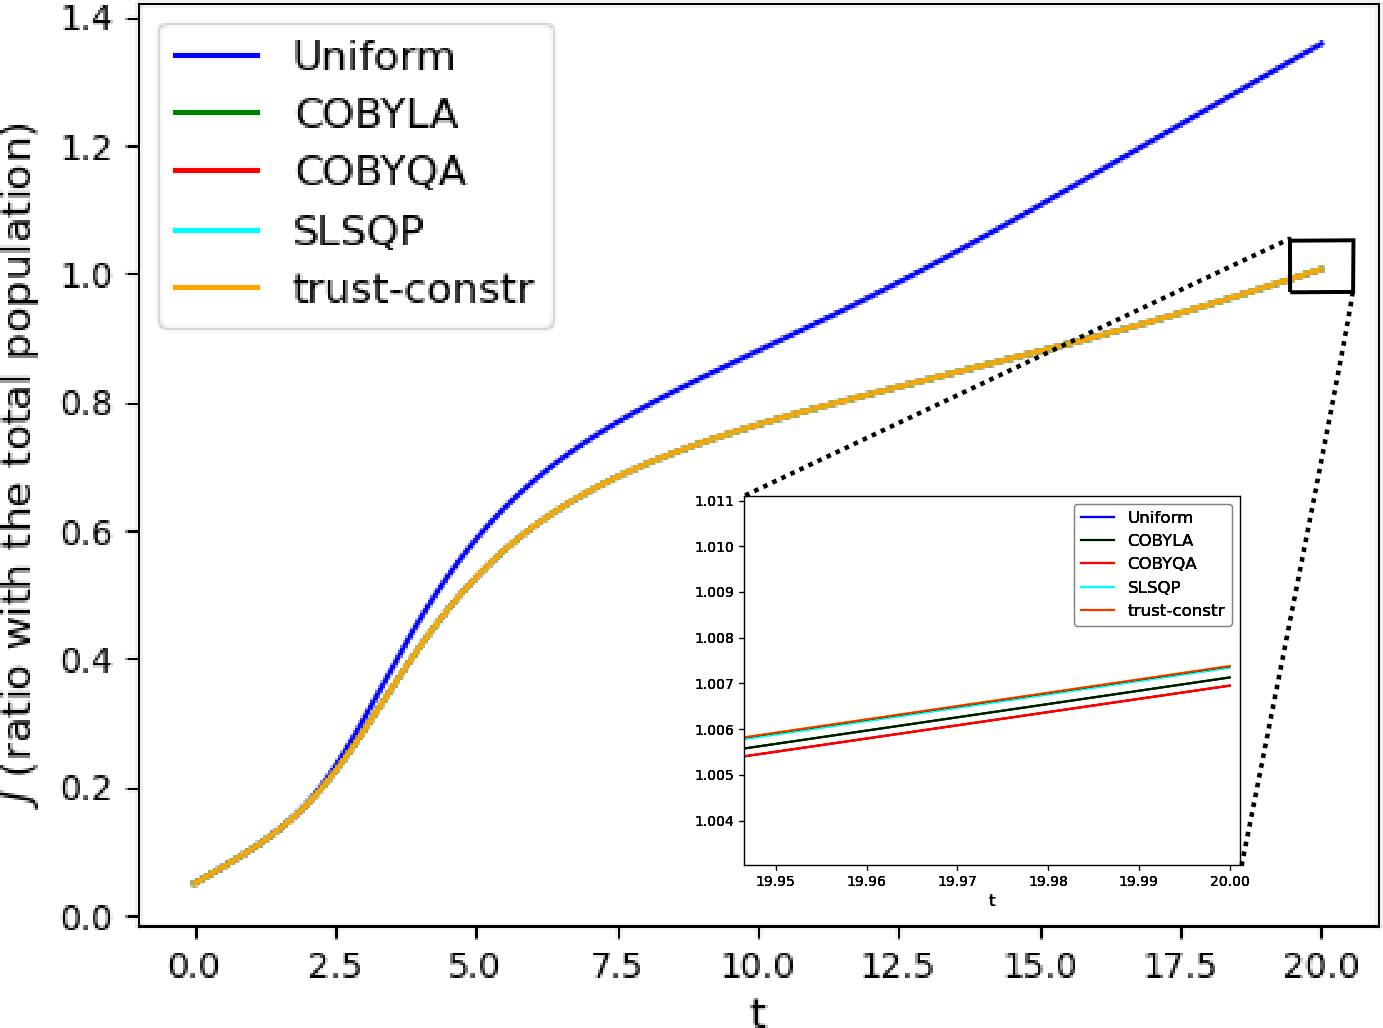
\includegraphics[scale=.15]{Imagenes/2x1-comparativa-metodos.png}
        % 2x1-comparativa-metodos.png: 1600x1200 px, 100dpi, 40.64x30.48 cm, bb=0 0 1152 864
        \caption{Methods Comparative}  \label{fig:resul2x1}
    \end{subfigure}
        \hfill
    \begin{subfigure}[t]{0.45\textwidth}
            %\centering
        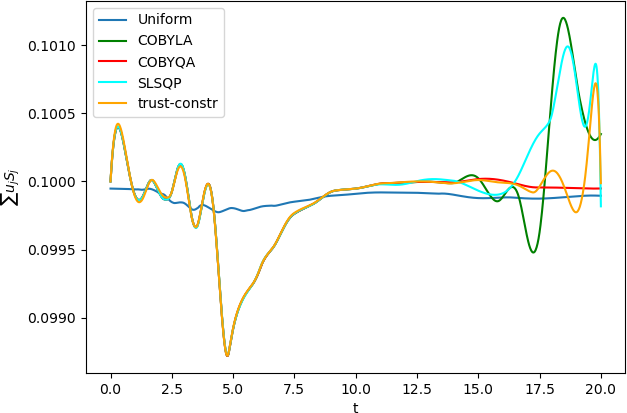
\includegraphics[scale=.35]{Imagenes/2x1-comparativa-metodos-restricciones.png}
        % 2x1-comparativa-metodos-restricciones.png: 949x480 px, 100dpi, 24.10x12.19 cm, bb=0 0 683 346
        \caption{Constrains satisfaction  $2\times 1$ network}
        \label{fig:restric2x1}
    \end{subfigure}
\\
    \vspace{0.5cm} % Espacio vertical entre filas
    \begin{subfigure}[b]{0.4\textwidth}
            %\centering
            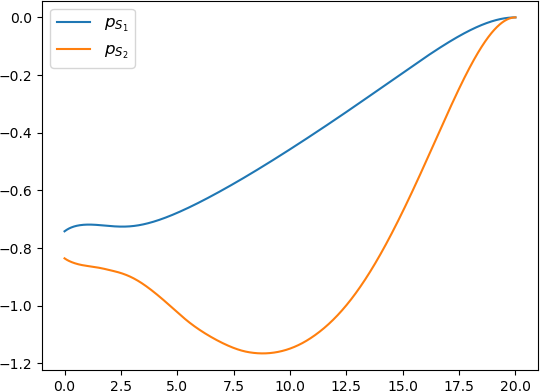
\includegraphics[scale=.4]{Imagenes/2x1-p_S.png}
            % 2x1-p_S.png: 640x480 px, 100dpi, 16.26x12.19 cm, bb=0 0 461 346
            \caption{Adjoint variables $p_S$}
            \label{fig:adjoint}
    \end{subfigure}
    \hfill
    \begin{subfigure}[b]{0.4\textwidth}
          %  \centering
        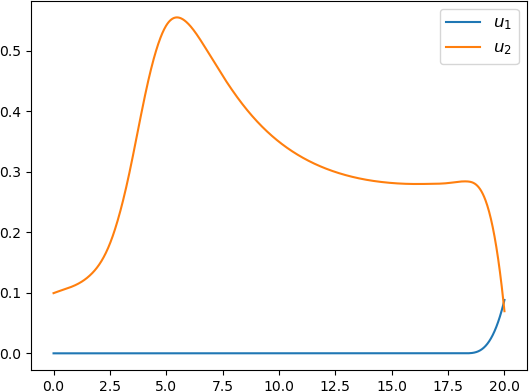
\includegraphics[scale=.4]{Imagenes/2x1-u.png}
        % 2x1-u.png: 640x480 px, 100dpi, 16.26x12.19 cm, bb=0 0 461 346
        \caption{Vaccination rates $u_i$}
        \label{fig:vaccination_rates}
    \end{subfigure}
    \caption{Results two nodes experiment.}\label{fig:result_2x2}
\end{figure}


The results are displayed in graphical form in the Figures \ref{fig:resul2x1}--\ref{fig:vaccination_rates}.  In Figure \ref{fig:resul2x1}, we plot the acummulated number of infected $J$ versus $t$. All numerical optimization algorithms show comparable performance, improving upon the uniform vaccination policy. It can also be observed (see Figure \ref{fig:restric2x1}) that all algorithms satisfy the constraints to the same order of accuracy. Figures \ref{fig:adjoint} and \ref{fig:vaccination_rates} are consistent with Proposition \ref{prop:cond_nec}; that is, all available vaccine stock at time $t$ is administered at node $i$, where $P_{S_i}$ equals the minimum of the vector $\mathbf{p_S}$.




\subsection{The experiment $5\times 5$ }



To test the capabilities of our algorithm, we addressed a larger-scale problem by considering networks with a large number of nodes. This leads to minimization problems with many degrees of freedom. Even for modest values of $k$ and $n$ ($k$ being the number of interpolation points and $n$ the number of nodes), the space over which we must minimize the objective function becomes very high-dimensional and challenging. We consider a metapopulations network of $25$ nodes (indicated with the set  $D=\{(r,s) \mid r,s=1,\ldots,5\}$), arranged in a $5 \times 5$ grid graph. In our model, individuals at node $(r,s)$ interact only with individuals at their nearest neighbors in the four cardinal directions (N, S, E, W). Naturally, nodes at the edges of the network have fewer neighbors. Nodes are enumerated with indices $i = 1, \ldots, 25$, assigned from top to bottom and left to right.\todo{quedamos aca}

 If $i$ and $j$  are neighbors  we assume that $\beta_{ij}=0.08$. We propose the following formula for intranode infection rates
 $$\beta_{ii}=1.1\left(\frac{2}{(r-5)^2+(s-5)^2+1}+1 \right),$$
 where $i$ corresponds to node $(r,s)$. Note that the intra-node infection rates range from $1.16$ to $3.3$, with the maximum value attained at the bottom-right node.


 We assume that $N_{i}=1$ for every $i=1,\ldots,25$, $\gamma=1$, $\mu=0.01$, $\alpha=0.2$.
 Finally, we assume that initially only node $i = 1$ contains infected individuals, with a total number equal to $0.1$. The function $M(t)$ was assumed to be constant and equal to 5\% of the total population, i.e., $M(t) = 0.05 \sum_{i=1}^{25} N_i = 1.25$.

As an initial guess, we adopt a uniform vaccination policy, where $u_j$ is independent of $j$, and set
 $$u_j(t)=\frac{M(t)}{\sum_{i=1}^{25}S_i(t)+\epsilon}.$$
The epsilon parameter in the formula is introduced to prevent infinite vaccination rates. In the experiments, it was set to $0.001$.



We will show the results obtained with the trust-constr algorithm, since it was the only one that produced a perceptible improvement over the initial candidate. In Figure \ref{fig:5x5_J}, we plot the cumulative number of infectious individuals corresponding to the two vaccination schemes: uniform and the result obtained with the trust-constr algorithm. We observe that the latter produces 8\% fewer cases of infection over the interval $[0,T]$ relative to the total population.
In Figure \ref{fig:5x5_restri}, we represent the total number of vaccinated individuals at time $t$, $\sum_{i=1}^nu_i(t)S_i(t)$, and observe that the result satisfactorily meets the restriction.


To study whether the conclusion of Proposition \ref{prop:cond_nec} is satisfied, we define $i_t=argmin(\bold{p_S}(t))$, we sort the vector $\bold{u}(t)$ from largest to smallest, and see what position, $j(t)$, occupies $i_t$  in that vector.  According to Proposition 5.1, the value of $j(t)$ should be 1. However, this does not occur, which is an indicator that the result of the algorithm is not an absolute minimum, but is presumably close to a local minimum. Nevertheless, we can observe a tendency for $j(t)$ to take small values. In Figure \ref{fig:5x5_chequeo}, we represent $j(t)$, and with the orange line the average value of $j(t)$, which is equal to $6.24$.


Figures \ref{fig:figura_con_subfiguras} and \ref{fig:figura_con_subfiguras2} present density diagrams for the variables $I$ and $uS$ at various time steps $t$.





\begin{figure}[h!]
    \centering
    % Fila 1
    \begin{subfigure}[t]{0.45\textwidth}
           % \centering
        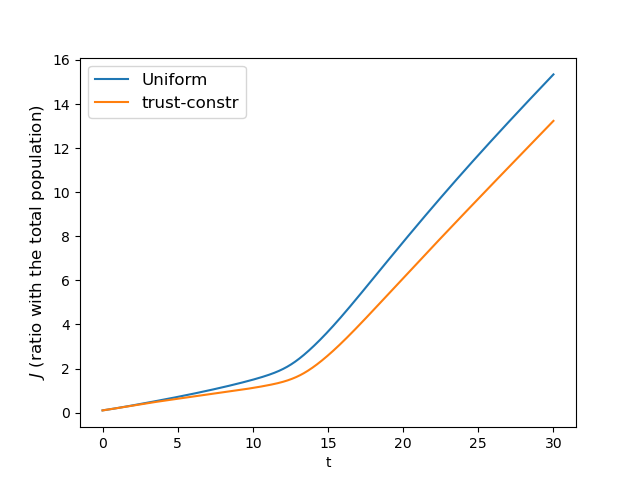
\includegraphics[scale=.4]{Imagenes/5x5-infeccion.png}
 % 5x5-infeccion.png: 640x480 px, 100dpi, 16.26x12.19 cm, bb=0 0 461 346
 \caption{Cumulative infected cases, for uniform and "optimal" vaccination}
 \label{fig:5x5_J}


    \end{subfigure}
        \hfill
    \begin{subfigure}[t]{0.45\textwidth}

 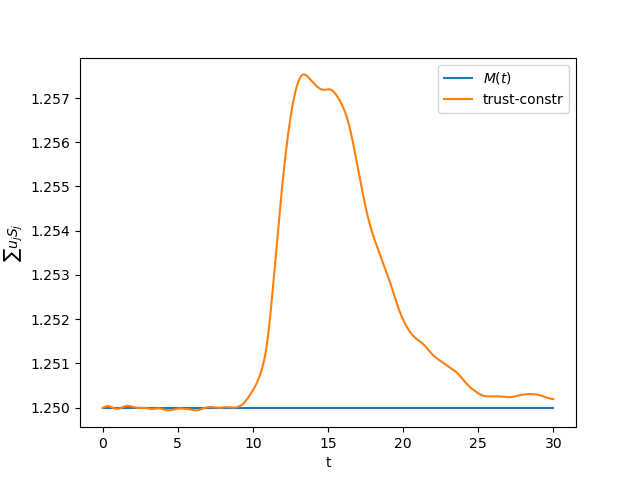
\includegraphics[scale=.4]{Imagenes/5x5-restriccion.png}
 % 5x5-restriccion.png: 640x480 px, 100dpi, 16.26x12.19 cm, bb=0 0 461 346
 \caption{Total vaccination}
 \label{fig:5x5_restri}

    \end{subfigure}
\end{figure}



\begin{figure}
 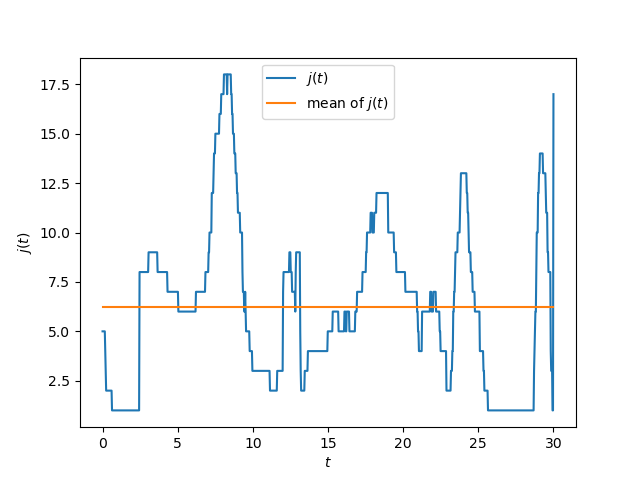
\includegraphics[scale=.6]{Imagenes/5x5-chequeo_teorema.png}
 \centering
 % 5x5-chequeo_teorema.png: 640x480 px, 100dpi, 16.26x12.19 cm, bb=0 0 461 346
 \caption{Graph of $j(t)$}
 \label{fig:5x5_chequeo}
\end{figure}


\begin{figure}[htbp]
    \centering
    % --- FILA 1 ---
    \begin{subfigure}[b]{0.48\textwidth}
        \centering
        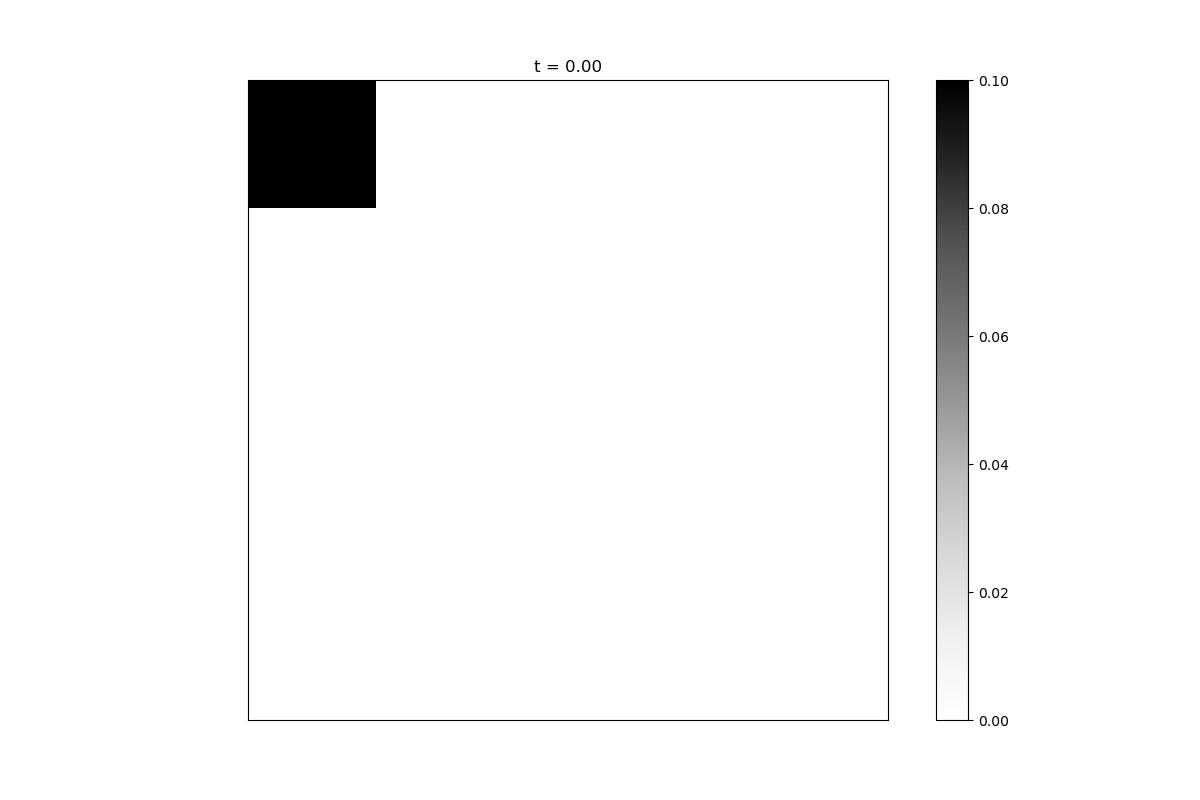
\includegraphics[width=\textwidth]{Imagenes/I00Control.png}
        \caption{Control $t=0$}
        \label{fig:subfig2}
    \end{subfigure}
    \hfill % Esto genera el espacio horizontal entre las dos fotos
    \begin{subfigure}[b]{0.48\textwidth}
        \centering
        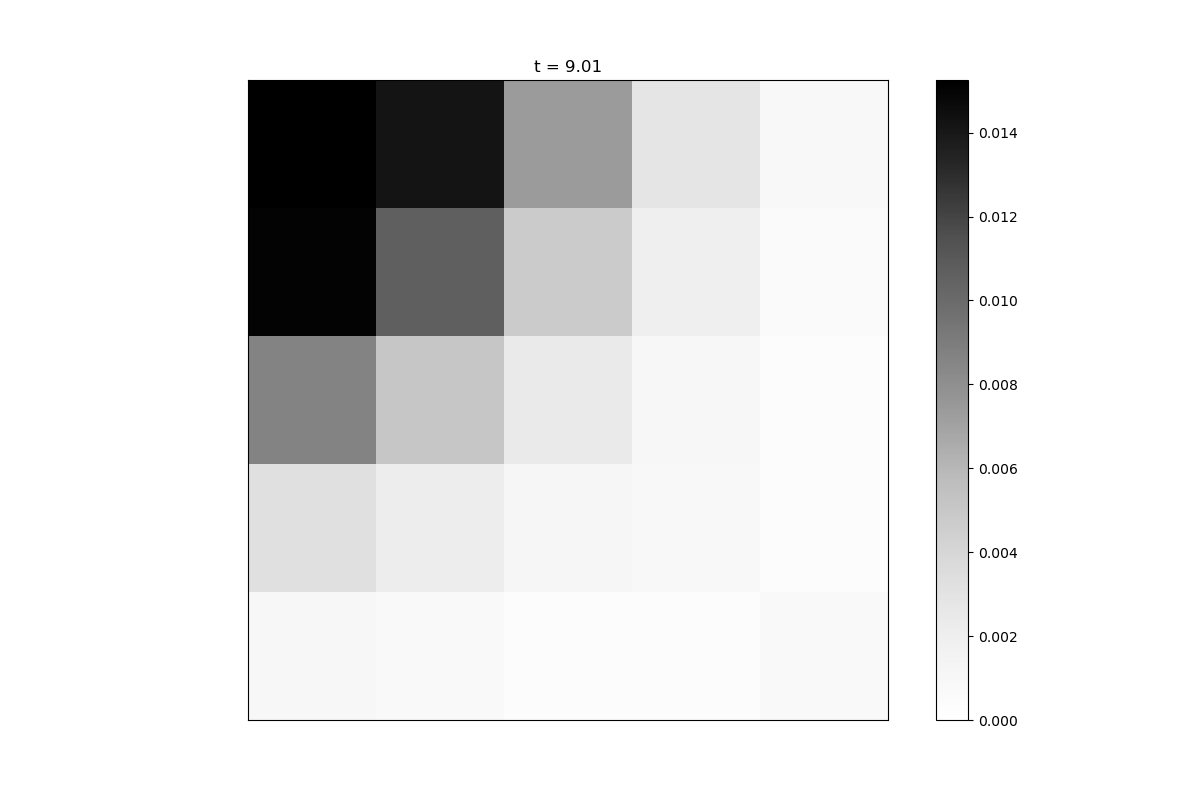
\includegraphics[width=\textwidth]{Imagenes/I03Control.png}
        \caption{Control $t=9.0$}
        \label{fig:subfig4}
    \end{subfigure}

    \vspace{0.5cm} % Espacio vertical entre filas

    % --- FILA 2 ---
    \begin{subfigure}[b]{0.48\textwidth}
        \centering
        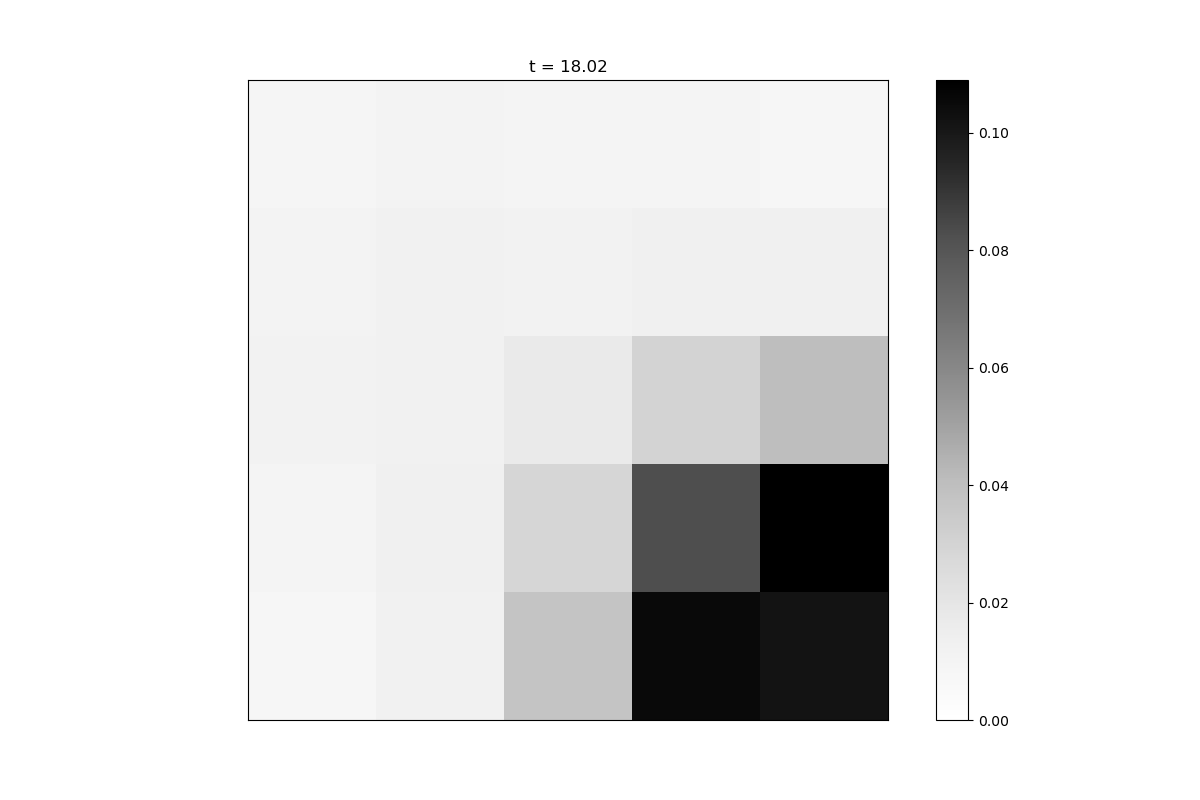
\includegraphics[width=\textwidth]{Imagenes/I06Control.png}
        \caption{Control $t=18.0$}
        \label{fig:subfig6}
    \end{subfigure}
    \hfill
    \begin{subfigure}[b]{0.48\textwidth}
        \centering
        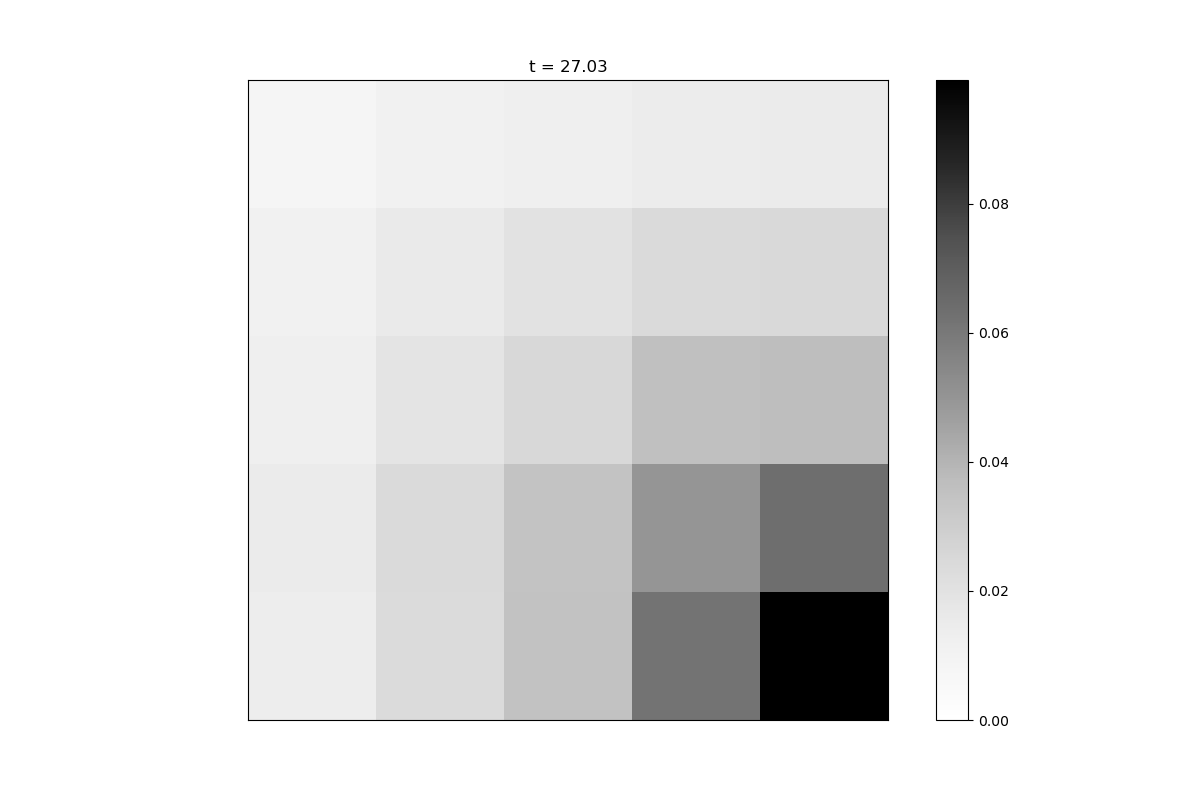
\includegraphics[width=\textwidth]{Imagenes/I09Control.png}
        \caption{Control $27.0$}
        \label{fig:subfig8}
    \end{subfigure}

    \caption{Evolution of the population of infected individuals in a  vaccination schedule  with optimal control.}
    \label{fig:figura_con_subfiguras}
\end{figure}

\begin{figure}[htbp]
    \centering
    % --- Fila 1 ---
    \begin{subfigure}[b]{0.45\textwidth}
        \centering
        \includegraphics[width=\textwidth]{Imagenes/u*S00Control.png}
        \caption{Control $t=0$}
        \label{fig:subfig2}
    \end{subfigure}
    \hfill % Empuja las imágenes a los extremos para que queden alineadas
    \begin{subfigure}[b]{0.45\textwidth}
        \centering
        \includegraphics[width=\textwidth]{Imagenes/u*S03Control.png}
        \caption{Control $t=9.0$}
        \label{fig:subfig4}
    \end{subfigure}

    \vspace{0.5cm} % Espacio vertical entre filas

    % --- Fila 2 ---
    \begin{subfigure}[b]{0.45\textwidth}
        \centering
        \includegraphics[width=\textwidth]{Imagenes/u*S06Control.png}
        \caption{Control $t=18.0$}
        \label{fig:subfig6}
    \end{subfigure}
    \hfill
    \begin{subfigure}[b]{0.45\textwidth}
        \centering
        \includegraphics[width=\textwidth]{Imagenes/u*S09Control.png}
        \caption{Control $t=27.0$}
        \label{fig:subfig8}
    \end{subfigure}

    \caption{Distribution of vaccines in the network under   optimally controlled vaccination schedules.}
    \label{fig:figura_con_subfiguras2}
\end{figure}



\section{Conclusions}

We studied a metapopulation SIR model with vaccination, which included demographic factors and a disease that only produced temporary immunity.  We considered variable vaccination rates given by the vector $\bold{u}(t)=(u_1(t), u_2(t),\ldots, u_n(t))$, where $u_i(t)$ is the vaccination rate on the $i$-patch. We identified a property of the transmission matrix that implies the spread of the disease to all patches of the metapopulation. We show that when $\bold{u}(t)=\bold{0}$, and under certain conditions, an endemic equilibrium appears.

We address an optimal control problem where we assume that the total number of individuals vaccinated per unit of time, i.e. $\sum_{i=1}^nu_i(t)S_i(t)$, cannot exceed a known function $M(t)$, which represents the availability of vaccines per unit of time at  $t$ moment. Under this constraint, we seek the function $\bold{u}(t)$ that produces the lowest number of total infected individuals over the time interval $[0,T]$. We show that this problem has a solution and, using Pontryagin's maximum principle, we see that the optimal solution takes the form of a bang-bang control. We designed a numerical method to solve the problem, and we implemented it, using python libraries, first to a metapopulation with two patches and then to a metapopulation with a transmission matrix based on a lattice graph. The numerical results show consistency with the theoretical results.




  \bibliographystyle{plain}
  \bibliography{control, epidemias, EpidemiologiaPapers,otros}

\end{document}
